\section{October 12, 2022}

\subsection{Subsection}

Let's start with an example.

\begin{example}
\exlabel

This is an example block. What happens when we do this example?
\end{example}

It turns out that this example gives us a \ac{nice property}, which we can emphasize using \verb+\ac+. Let's introduce a definition.

\begin{definition}
\deflabel

This is a definition.
\end{definition}

Using our definition, we can make a nice diagram:
\begin{center}
\begin{asy}
import graph; size(5cm); 
pen dps = linewidth(0.7) + fontsize(9); defaultpen(dps);
pen dotstyle = 2+black;
real scale = 2.25;
DefaultHead.size=new real(pen p=currentpen) {return 4bp;};

pair O = (0,0);
pair A = scale(1.5)*dir(45);
pair C = scale(0.5)*dir(225);
pair b = dir(20);
pair Ab = dir(70);

draw(O--A, Arrow);
draw(O--C, Arrow);
draw(O--b, Arrow);
draw(O--Ab, Arrow);
draw(Ab--b, Arrow);

/* dot(O,dotstyle); */ 
label("$Ab$", Ab, W*scale);
label("$b$", b, S*scale);
label("$(Ab+b)/2$", A, NE*scale);
label("$(b-Ab)/2$", b, NE*scale);
\end{asy}
\end{center}

Some more example diagrams and templates are available at the bottom of \verb+_andrew.sty+. These include tables, common matrix patterns, asymptote starters, and other useful templates to copy and paste that help with taking notes in real time. 

Using these properties, this leads us to our first theorem:

\begin{theorem}
\thmlabelname{Important Theorem}

This is the statement for our theorem. 
\end{theorem}

\begin{proof}
You can use proof environments as usual. 
\end{proof}

Let's say we wanted to state a theorem without a name. Then, we could use \verb+\thmlabel+ instead of \verb+\thmlabename+ inside of our theorem box. 

\subsection{Another Subsection}

Our theorem leads to some nice results. For example, consider the following. \comment{Add functionality for theorem referencing}.

\begin{theorem}
\corlabel

This is a corollary. You may also find \verb+proplabel+ useful for propositions. 
\end{theorem}

Finally, make sure that you do not conflate these two concepts:

\begin{misconception}
\mislabel

This is a common misconception. Make sure not to fall into this trap. 
\end{misconception}

Have fun!
\begin{figure}[h]
    \centering
    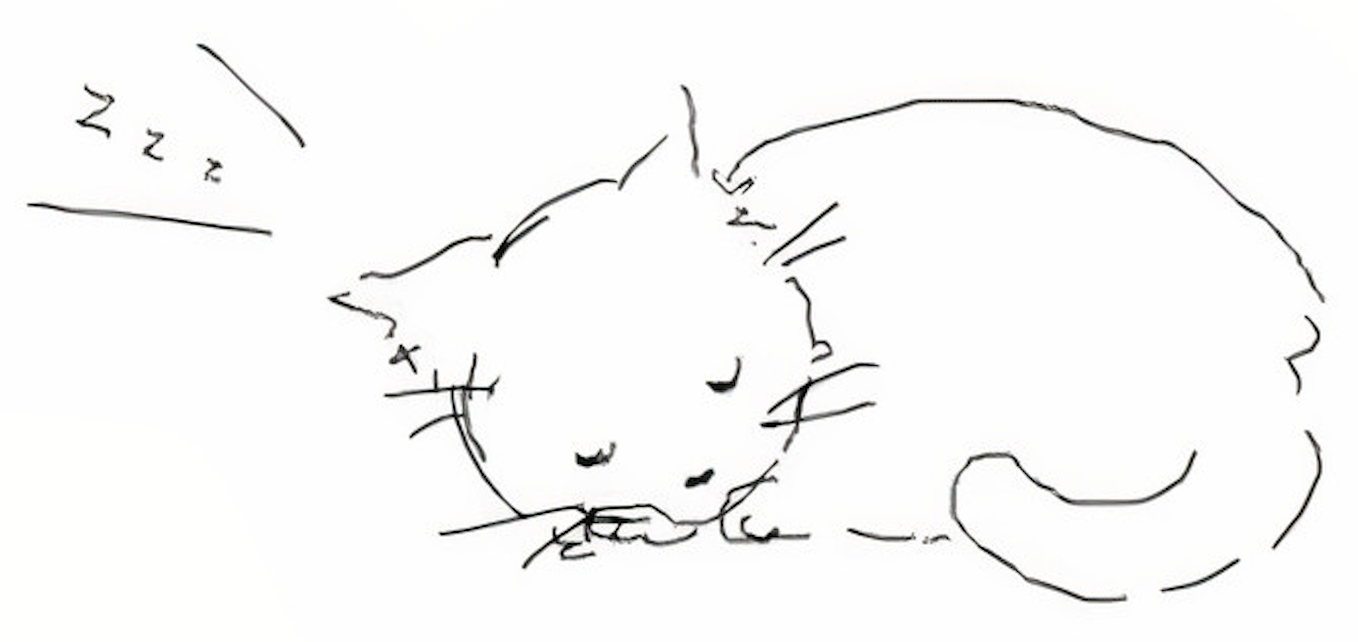
\includegraphics[width=6cm]{images/sleepingcat.png}
    \caption{Sleeping Cat}
\end{figure}

